\documentclass[11pt,a5paper]{article}

\usepackage[T1]{fontenc}
\usepackage[utf8]{inputenc}
\usepackage{lmodern, microtype}
\usepackage[estonian]{babel}

\usepackage{siunitx}
\sisetup{inter-unit-product=\ensuremath{{}\cdot{}}, per-mode=fraction, exponent-product=\cdot, output-decimal-marker={,}}

\usepackage{graphicx}
\usepackage{wrapfig}
\usepackage{subfig}
\usepackage{tikz}
\usetikzlibrary{patterns, patterns.meta}
\usetikzlibrary{arrows.meta}
\usepackage[european]{circuitikz}
\tikzset{component/.style={draw,thick,circle,fill=white,minimum size=0.75cm,inner sep=0pt}}
\usepackage{amsmath,amssymb}
\usepackage{amsfonts}
\usepackage[hidelinks]{hyperref}
\usepackage{csquotes}
\usepackage{caption}
\usepackage{enumitem}
\usepackage{wrapfig}
\topmargin=-3.0cm \textheight=19cm \textwidth=12.9cm
\oddsidemargin=-1.5cm  \evensidemargin=-1.5cm
\setlength{\parindent}{0pt} \setlength{\parskip}{6pt} \sloppy
\sloppy \relpenalty=10000 \binoppenalty=10000
\pagestyle{empty}

\newcommand{\numb}[1]{\vspace{5pt}\textbf{\large #1}}
\newcommand{\nimi}[1]{(\textsl{\small #1})}
\newcommand{\punktid}[1]{(\emph{#1~p.})}
\newcounter{ylesanne}
\newcommand{\yl}[1]{\addtocounter{ylesanne}{1}\numb{\theylesanne.} \nimi{#1} \newblock{}}
\newcommand{\autor}[1]{}% Kasuta võistluse ajal
%\newcommand{\autor}[1]{\emph{ Autor: #1}}% Kasuta kui vaja autorit

\begin{document}
\begin{center}
  \textbf{\Large Eesti koolinoorte 34.\ füüsika lahtine võistlus} \par
  \emph{2.\ detsember 2023. a.\\Vanema rühma ülesanded (11.--12.\ klass)}
\end{center}

\resizebox{\textwidth}{!}{
  \emph{%
    \begin{tabular}{@{}l@{}}
      \textbf{Palun kirjutada iga ülesande lahendus eraldi lehele.}\\
      Lahendamisaeg on 5 tundi. \\
      Iga osavõtja võib lahendada kõiki pakutud ülesandeid. \\
      Arvesse lähevad 6 suurima punktide arvu saanud lahendust. \\
      Kasutada võib kirjutus- ja joonestusvahendeid ning kalkulaatorit. Muud abivahendid on keelatud.\\
    \end{tabular}
  }
} \par



\yl{PAVILJON}
Mirtel varjus vihma eest paviljoni. Sellel seinteta paviljonil on ruudukujuline põrand küljepikkusega $a = \SI{5}{\meter}$, mida varjab postidele toetuv põrandaga ühesuurune ruudukujuline lame katus, mille kõrgus maapinnast $H=\SI{3}{\meter}$. Mirtel märkas, et 20\% põranda pindalast on siiski märg, sest sinna langevad vihmapiisad. Ta tegi anemomeetri abil kindlaks, et puhub konstantse suunaga tuul, mille kiirus $v_t = \SI{3}{\meter\per\second}$ on kõikjal üks ja sama. Mida on nende andmete põhjal võimalik öelda piiskade vertikaalkiiruse kohta: milline on selle suurim võimalik väärtus $v_{max}$ ja vähim võimalik väärtus $v_{min}$?
Minimaalsuse ja maksimaalsuse ranget tõestust pole vaja esitada.
\punktid{6} \autor{Uku Andreas Reigo}



\yl{KUMERPEEGEL}
Joonisel (suurendatult lisalehel) on kujutatud ese AB ja kumerpeegel, mille keskpunkt on O ja fookus on F. Eeldame, et ese on sümmeetriateljest natuke nihkes, nii et see on punktist P nähtav nii otse kui kumerpeeglis. Mitu korda väiksem paistab ese AB punktist P kumerpeegli abil vaadelduna (võrreldes otse vaatamisega)? Lahendage ülesanne lisalehel.
\punktid{6} \autor{Richard Luhtaru}

\begin{figure}[h]
    \centering

    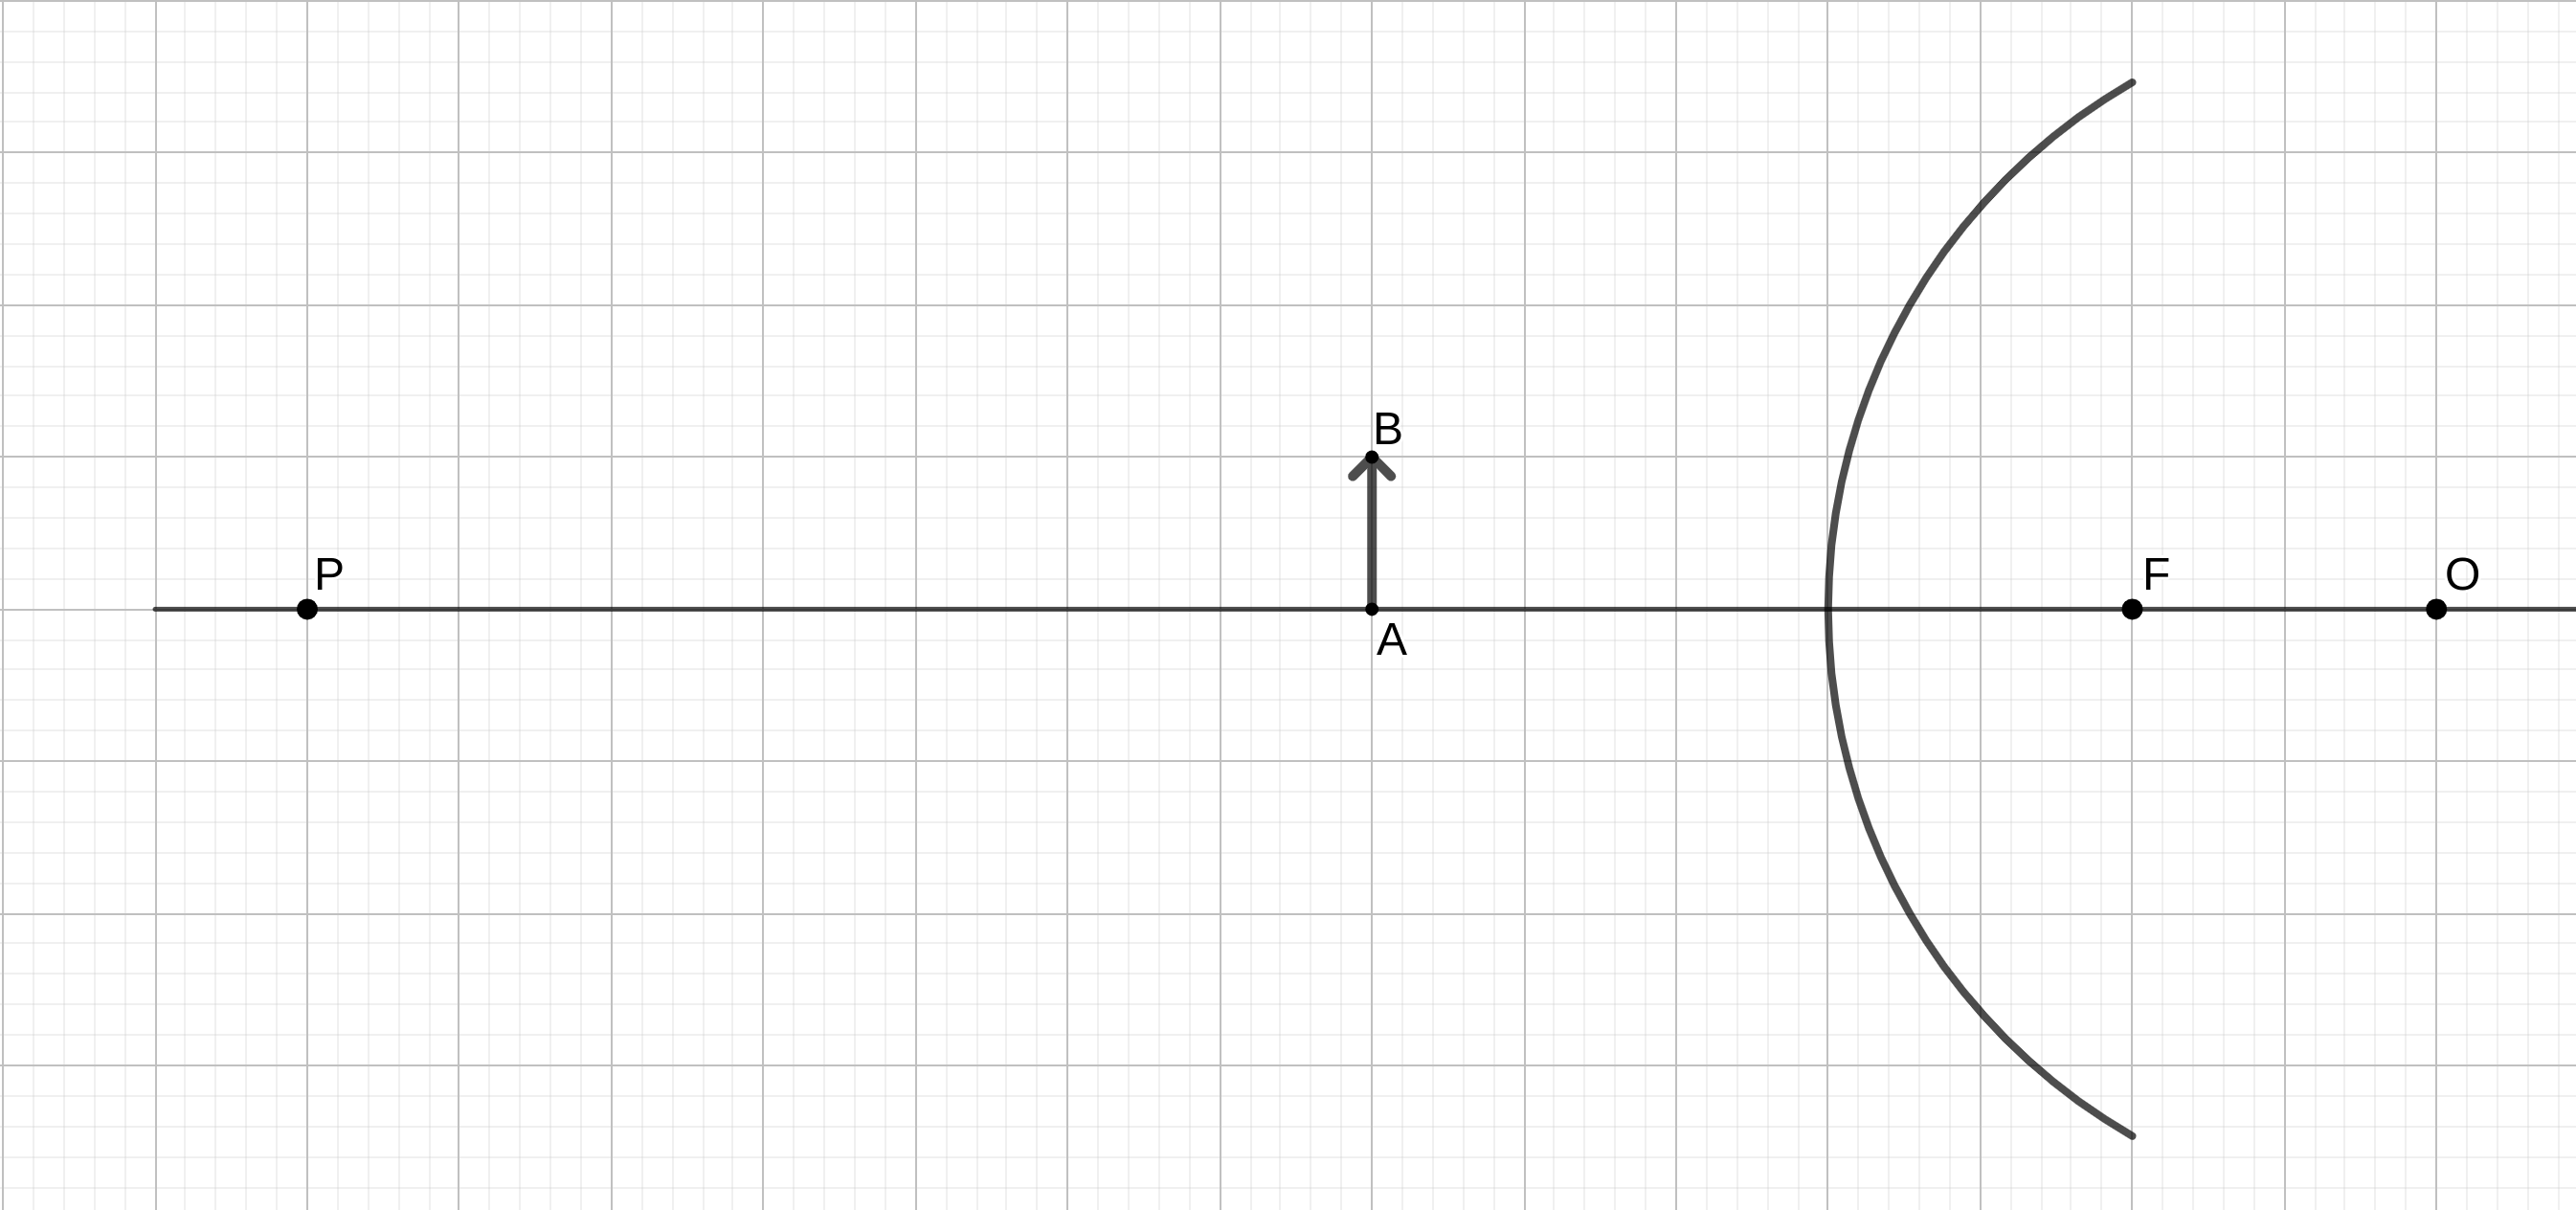
\includegraphics[width=0.75\linewidth]{kumerpeegel_joonis.png}
     \vspace{-20pt}
\end{figure}


\newpage



\begin{wrapfigure}[8]{r}{0.5\linewidth}
    %\vspace{-10pt}
    \begin{center}
        \vspace{5pt}
        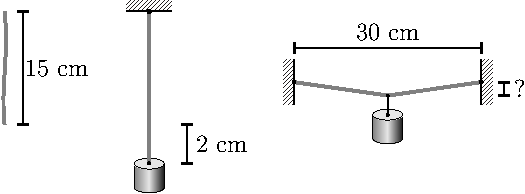
\includegraphics[width=\linewidth]{kummipael_joonis.pdf}
    \end{center}
\end{wrapfigure}


\yl{KUMMIPAEL}
Kummipaela pikkus vabas olekus on $L=\SI{15}{cm}$. Kui kummipaela külge riputati tundmatu massiga koormis, siis kummipaela pikkus kasvas $\Delta L=\SI{2}{cm}$ võrra (vt joonis). Seejärel kummipael fikseeriti otstest kahe samal kõrgusel paikneva punkti vahele, mille vahekaugus oli $2L$ (st pael venitati $L$ võrra pikemaks). Sama koormis riputati nüüd kummipaela keskpunkti. Hinnake, kui suur on selle punkti läbivajumine. Võib eeldada, et kummipaelas tekkiv elastsusjõud on võrdeline pikenemisega ja kummipaela enda mass on tühine.\\ \emph{Märkus:} Väikeste nurkade $x$ korral võib kasutada lähendust $\sin{x} \approx \tan{x} \approx x$ (nurk $x$ on radiaanides).
\punktid{8} \autor{Valter Kiisk}









\begin{wrapfigure}{r}{0.19\textwidth}
\vspace{-0.8cm}
  \begin{center}
    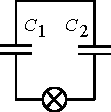
\includegraphics[width=1\linewidth]{kondekad_joonis.pdf}
    %\caption{}
  \end{center}
  \vspace{-0.9cm}
\end{wrapfigure}

\yl{KONDENSAATORID}
Indrekul on kaks kondensaatorit mahtuvustega $C_1=40\,\mu$F ja $C_2=60\,\mu$F. Esimene neist ($C_1$) on laetud pingeni $U_0$ = 15 kV ja teine ($C_2$) on pingeta. Indrek soovib teist kondensaatorit esimese abil laadida, aga kardab, et laadimisjuhtmed süttivad suure voolutugevuse tõttu. Selle vältimiseks lisab ta ahelasse hõõglambi (vt joonis). Kui suur soojushulk eraldub  kogu süsteemis, kui Indrek hoiab kondensaatoreid ühenduses pikka aega?
\punktid{8} \autor{Päivo Simson}





\yl{ELEKTRIAUTO}
Gaafikul on kujutatud teatava elektriauto mootori kasuliku mehaanilise võimsuse sõltuvus kiirusest. Auto mass on $m=\SI{2200}{kg}$.\\
\osa Milline on suurim võimalik kiirendus?\\
\osa Minimaalselt kui kaua aega kulub 100 km tunnikiiruse saavutamiseks?\\
Õhutakistust ja rehvi libisemist teekattel võib ignoreerida.
\punktid{10} \autor{VALTER KIISK}


\begin{figure}[h]
    \centering
    \vspace{-10pt}
    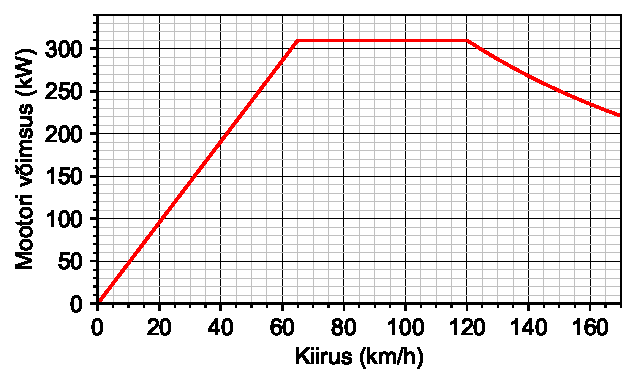
\includegraphics[width=0.75\linewidth]{elektriauto_joonis.pdf}
    \vspace{-35pt}
\end{figure}

\newpage

\yl{VÕIMAS MOOTOR}
K20A on 4-taktiline, 4-silindriline, \SI{2,0}{\liter} mootor (iga silindri maht on \SI{0,5}{\liter}), mis saavutab oma tippvõimsuse $f= \SI{8000}{\per\minute}$ (pööret/min) juures. Üks takt kestab pool pööret, taktid on: sisselasketakt, survetakt, töötakt ja väljalasketakt.
Temperatuuril $T_1=\SI{20}\celsius$ on õhu tihedus $\rho=\SI{1.2}{\kg\per\m\cubed}$; kui välistemperatuur on $T_1$, siis on sissevõtutakti lõpus silindris oleva õhu temperatuur $T_2=\SI{60}\celsius$.  Sissevõtutakti lõpus kolbi pritsitud bensiini ruumalaga mitte arvestada. Leidke sellise mootori tippvõimsus.
Bensiini energiatihedus on $\epsilon = \SI{46}{\mega\joule\per\kilogram}$, ideaalne kulunud õhu ja bensiini suhe on $\gamma = \frac{\SI{14,7}{\gram}}{\SI{1}{\gram}}$. Võib eeldada, et toimub täielik põlemine. Mootori efektiivsus on $\eta=37\%$.
\punktid{10} \autor{Marten Rannut}





\yl{SOOJUSPUMP} 
Hilissügisel maamajja minnes on nii õues kui toas $T_0=\SI {2}{\celsius}$ sooja. Kui soojuspump sisse lülitada, kulub toas keskmise temperatuur  tõusmiseks $T_1=\SI {4}{\celsius}$-ni $t_0=\SI{30}{\min}$. Kui soojuspump jääkski pidevalt töötama, tõuseks temperatuur toas lõpuks $T_f=\SI {42}{\celsius}$-ni. Paraja soojuse tagamiseks lülitab soojuspumpa sisse ehitatud termorelee pumba välja, kui toatemperatuur tõuseb üle $T_3=\SI{23}\celsius$ ning uuesti sisse tagasi, kui temperatuur langeb alla $T_2=\SI{22}{\celsius}$. Kui pikk on ajavahemik kahe järjestikuse sisse lülitumise vahel? Eeldage, et soojuspumba kütmisvõimsus on kogu aeg üks ja sama. Lahendamisel võib teha täiendavaid mõistlikke lähendusi.\\ \emph{Märkus:} Võite eeldada, et soojuskadu on võrdeline temperatuuride vahega.
\punktid{10} \autor{Jaan Kalda}




\begin{wrapfigure}[8]{r}{0.2\linewidth}
    \vspace{-30pt}
    \begin{center}
        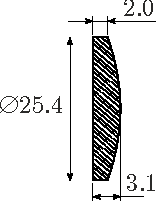
\includegraphics[width=\linewidth]{tasakumer-laats}
    \end{center}
\end{wrapfigure}
\yl{LÄÄTS} 
Joonisel on kujutatud teatava tasakumera läätse ristlõige ja selle mõõdud millimeetrites. Lääts on valmistatud klaasist, mille murdumisnäitaja $n=\num{1.52}$.\\
\osa Eeldusel, et kumerpind on sfääriline, kui suur on selle kõverusraadius?\\
\osa Määrake läätse fookuskaugus kiirte jaoks, mis kulgevad optilise peatelje lähedal (Võite eeldada, et lääts on õhuke, st piisab 3 mm täpsusega õigest vastusest.)! \\ \emph{Märkus:} Väikeste nurkade $x$ korral võib kasutada lähendust $\sin{x} \approx \tan{x} \approx x$ (nurk $x$ on radiaanides).
\punktid{10} \autor{Valter Kiisk}

\newpage
\begin{wrapfigure}[8]{r}{0.4\linewidth}
    \vspace{-25pt}
    \begin{center}
        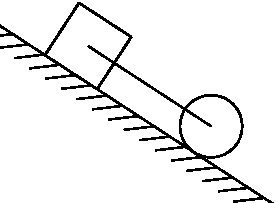
\includegraphics[width=\linewidth]{klots-silinder}
    \end{center}
\end{wrapfigure}
\yl{KLOTS JA SILINDER}
Anul on samasuguse läbimõõdu ja massiga pikk silinder ja klots. Ta lasi silindril mäenõlvast alla veereda ning mõõtis ajaks $t_1 = \SI{5}{\second}$. Seejärel lasi ta klotsil alla libiseda ning sai ajaks $t_2 = \SI{7}{\second}$. Kui palju kuluks silindril ja klotsil mäest alla jõudmiseks, kui need joonisel näidatud moel liigesega ühendada? Võib eeldada, et mäenõlv on ühtlase kaldenurgaga, hõõrdejõud kõikide pindade vahel on konstantne, silinder veereb alati libisemata ning et igas stenaariumis läbisid objektid sama vahemaa. Silindri inertsimoment on $I=mR^2/2$, kus $m$ on silindri mass ja $R$ selle raadius. Õhutakistusega mitte arvestada.
\punktid{12} \autor{Taavet Kalda}









\newcommand{\magnetvali}{
    \begin{tikzpicture}[scale=0.70]
        \draw (-4,0) -- (4,0);
        \draw (0,-4) -- (0,4);

        \draw[thick,->] (0,2) node [anchor = east] {$(0,h)$}
                            -- ++(60:1.6)
                            node [midway, anchor = west] {$\Vec{v}$};
        \draw (0,2) -- ++ (60:1) node [midway, anchor = south east, xshift = 6] {$\alpha$}
            arc (60:90:1);

        \draw (-2,2) circle (0.25) node[above, anchor = south, yshift = 5] {$B_1$};
        \filldraw (-2,2) circle (0.05);
        
        \draw (2,-2) circle (0.25) node[above, anchor = south, yshift = 5] {$B_1$};
        \filldraw (2,-2) circle (0.05);

        \draw (2,2) circle (0.25) node[above, anchor = south, yshift = 5] {$B_2$};
        \draw (2.25,2) -- (1.75,2);
        \draw (2,1.75) -- (2,2.25);

        \draw (-2,-2) circle (0.25) node[above, anchor = south, yshift = 5] {$B_2$};
        \draw (-2.25,-2) -- (-1.75,-2);
        \draw (-2,-1.75) -- (-2,-2.25);
        
    \end{tikzpicture}
} 

\setlength{\columnsep}{20pt}
\begin{wrapfigure}{r}{0pt}
    \vspace{-50pt}
    \raisebox{-50pt}[0.5\dimexpr\height][-10000pt]{\magnetvali{}}    
    \vspace{-500pt}
\end{wrapfigure}



\yl{KÕVER TRAJEKTOOR}
Elektron massiga $m$ ja laenguga $q$ alustab liikumist punkis $(0,h)$ kiirusega $v$ (vt joonis), kusjuures kiirusvektori ja y-telje sihi vaheline nurk on $\alpha$ nii, et $0<\alpha<\frac{\pi}{4}$. Milline peab olema magnetväljade tugevuste suhe $\frac{B_1}{B_2}$, et elektroni edasine trajektoor oleks kinnine ning ennast mitte lõikav?
\punktid{12} \autor{Uku Andreas Reigo}

\end{document}
